\chapter{演化的证据}\label{ch:g9:evidence-of-evolution}

本书两次停在一个重大论断的边缘：
\omterm{prop:g6:classification-kinship:kinship}{亲缘关系}树的\omterm{def:g1:plants-around-us:tree}{分支}终将汇合
（\cref{rem:g6:classification-kinship:implies}），而每种\omterm{def:g6:exploring-our-environment:components}{生物}
都读取同一套\omterm{def:g9:heredity-and-traits:heredity}{遗传}密码
（\cref{rem:g9:genes-and-dna:universal}）。它们所指向的论断
有一个名字——\emph{演化}：\omterm{def:g5:biodiversity:species}{物种}会跨代改变，
所有\omterm{def:g5:biodiversity:species}{物种}都源于共同祖先。
在下一章追问\emph{如何}之前，本章先做
\cref{exo:g6:classification-kinship:12}所要求的事：
陈列证据。

\section{岩石的见证}

\begin{definition}[化石]\label{def:g9:evidence-of-evolution:fossils}
\emph{化石}\index{化石}是保存下来的过去生命的痕迹——
贝壳、\omterm{def:g3:bones-and-muscles:skeleton}{骨骼}、叶印、足迹，都封存于
沉积岩中。岩层按时间顺序叠置，最老的
在最下层；自下而上读岩层，就是读历史。化石
属于\cref{def:g6:exploring-our-environment:components}所列清单中的
遗存那一半，
能保存数百万年。
\end{definition}

\begin{proposition}[岩层记录显示了什么]\label{prop:g9:evidence-of-evolution:record}
按顺序阅读，记录共提供三类证据：
\begin{enumerate}
  \item \emph{\omterm{def:g1:animals-around-us:animal}{动物}群随时代更替}：每个地层时代都有其独特的
        \omterm{def:g1:animals-around-us:animal}{动物}群成员——三叶虫层中没有兔子，
        兔子所在地层中也没有三叶虫；深层地层中的大多数\omterm{def:g5:biodiversity:species}{物种}
        都已\emph{\omterm{prop:g5:biodiversity:loss}{灭绝}}
        （\cref{prop:g5:biodiversity:loss}中的用语，
        此处还包含漫长的地质时间背景）；
  \item \emph{层序与树状结构一致}：\omterm{prop:g3:sorting-living-things:groups}{鱼类}出现在
        较深地层中，四足两栖类的近亲位于其上，
        爬行类近亲再上，\omterm{prop:g3:sorting-living-things:groups}{哺乳动物}与\omterm{prop:g3:sorting-living-things:groups}{鸟类}
        位置更高——分类体系中的各个分类框
        （\cref{pb:g6:classification-kinship:1}）在时间上
        依序堆叠，正如\omterm{prop:g6:classification-kinship:kinship}{亲缘关系}所预言；
  \item \emph{过渡类型确实存在}：著名的
        \emph{Archaeopteryx}\omterm{def:g9:evidence-of-evolution:fossils}{化石}板——\omterm{def:g1:animals-around-us:covering}{羽毛}与翅膀长在
        有齿、长骨尾的爬行类骨架上——
        正位于\omterm{prop:g3:sorting-living-things:groups}{鸟类}与爬行类\omterm{def:g1:plants-around-us:tree}{分支}分开之处；\omterm{def:g9:evidence-of-evolution:fossils}{化石}
        具有可用后肢的\omterm{def:g9:evidence-of-evolution:fossils}{化石}鲸，正处于
        \cref{ex:g6:classification-kinship:whale}所要求的
        陆生\omterm{prop:g3:sorting-living-things:groups}{哺乳动物}祖先所要求的环节。
\end{enumerate}
\end{proposition}
\admitted

\begin{example}[鲸类系列]\label{ex:g9:evidence-of-evolution:whales}
鲸的历史档案由岩石补全：相继出土的\omterm{def:g9:evidence-of-evolution:fossils}{化石}，
按时间顺序排列，始于一种狼大小的四足陆栖\omterm{prop:g3:sorting-living-things:groups}{哺乳动物}，
经由腿渐缩、尾渐强的类型，
终至无腿的完全水生\omterm{def:g1:animals-around-us:animal}{动物}——
而现今的鲸仍保有细小隐藏的髋骨与腿骨，
（\cref{ex:g6:classification-kinship:placing}曾提到这些
残迹），仍哺育幼崽、\omterm{def:g7:what-is-respiration:respiration}{呼吸}空气，并长着
胎毛。预测、\omterm{def:g9:evidence-of-evolution:fossils}{化石}与残迹：三把钥匙，
开同一把锁。
\end{example}

\begin{omfigure}
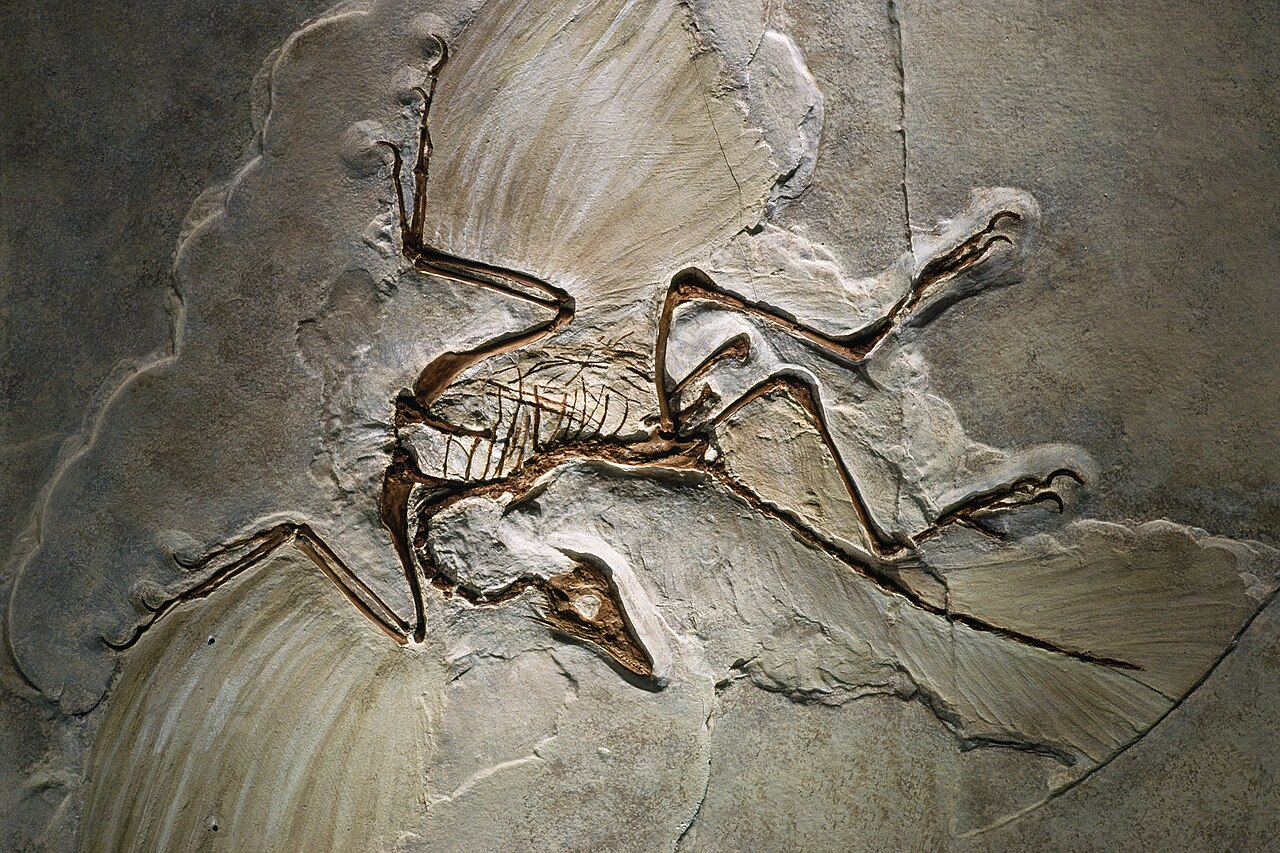
\includegraphics[width=0.62\linewidth]{images/book1/archaeopteryx.jpg}

{\small 一件\emph{Archaeopteryx}\omterm{def:g9:evidence-of-evolution:fossils}{化石}：带\omterm{def:g1:animals-around-us:covering}{羽毛}的翅膀长在
有齿、长尾的爬行类骨架上——一种过渡类型，
位于\omterm{def:g6:classification-kinship:tree}{亲缘树}\omterm{def:g1:plants-around-us:tree}{分支}分开之处。}
\end{omfigure}

\section{生物体的见证}

\begin{proposition}[解剖结构保存历史]\label{prop:g9:evidence-of-evolution:anatomy}
\omterm{def:g6:exploring-our-environment:components}{生物}体承载着自身的历史：
\begin{itemize}
  \item \emph{共同的结构蓝图}：蝙蝠的翼、鲸的鳍状肢、
        马的腿和你的手臂，同属一种\omterm{def:g3:bones-and-muscles:skeleton}{骨骼}排布
        （\cref{pb:g6:classification-kinship:1}中
        \omterm{def:g1:my-body:parts}{四肢}分叉）经拉长、缩短，并改作他用
        ——\omterm{def:g9:heredity-and-traits:heredity}{遗传}能够解释全新设计
        绝不会重复的结构；
  \item \emph{残迹}：鲸的髋骨，无法飞行的
        甲虫闭合不用的翅、你自己的尾骨和
        阑尾退化的状态——这些部分之所以保留，
        是因为祖先结构是在其上改造，而非白手起家；
  \item \emph{\omterm{def:g5:human-reproduction:pregnancy}{胚胎}相似}：鱼、鸡与人的\omterm{def:g4:classifying-animals:vertebrate}{脊椎动物}\omterm{def:g5:human-reproduction:pregnancy}{胚胎}
        在最初的
        数周里惊人地相似
        （\cref{prop:g8:from-egg-to-birth:timetable}中的蓝图奠定）——
        共同的构建指令，
        后期才分道扬镳。
\end{itemize}
\end{proposition}
\admitted

\begin{proposition}[分子投票]\label{prop:g9:evidence-of-evolution:molecules}
最新的证据是
\cref{rem:g9:genes-and-dna:universal}中的密码。比较各\omterm{def:g5:biodiversity:species}{物种}间
同一保守\omterm{def:g9:genes-and-dna:gene}{基因}的“拼写”：人与黑猩猩
相差字母较少，人与小鼠相差较多，人与
鱼相差更多，人与\omterm{ex:g6:producing-our-food:bread}{酵母}相差最多——而
这些距离逐个\omterm{def:g9:genes-and-dna:gene}{基因}累计统计，重新绘出了
\emph{同一棵树}——解剖学家据\omterm{def:g3:bones-and-muscles:skeleton}{骨骼}绘制的，
古生物学家据地层绘制的。三条独立的证据，
指向同一棵\omterm{def:g6:classification-kinship:tree}{亲缘树}：这种吻合，使生物学家
不再争论\emph{是否}，而转向\emph{如何}。
\end{proposition}
\admitted

\begin{example}[观察变化]\label{ex:g9:evidence-of-evolution:live}
在世代更替迅速的地方，变化甚至可以被直接观察到。
桦尺蛾的深色型在被煤烟熏黑的工业林中\omterm{def:g6:how-plants-spread:dispersal}{扩散}，
空气变清洁后便随之减少；
抗杀虫剂的\omterm{prop:g3:sorting-living-things:groups}{昆虫}与耐抗生素的\omterm{def:g6:producing-our-food:fermentation}{微生物}
（\cref{ch:g9:microbes-and-infection}将讨论其医学病例）
数年之内即可出现；岛雀的
喙大小分布随干旱与丰裕而变化，
由套环与卡尺的野外研究实时测得。小幅变动，
历时短暂——机制被当场捕捉，
不论其长远影响如何。
\end{example}

\begin{method}[权衡历史证据]\label{met:g9:evidence-of-evolution:weigh}
演化即历史，历史性论断须经检验，
正如
\cref{pb:g9:unique-individuals:1}中的悬案——依靠
独立证据的相互印证：
\begin{enumerate}
  \item 问该论断\emph{预言}了什么：哪些
        中间产物、哪些痕迹器官、
        哪些分子距离；
  \item 逐一核查每条证据：岩石、躯体、
        分子与实时观察；
  \item 权衡其独立性：不可能相互串通的证据，
        若彼此吻合，
        则可信度成倍增加；
  \item 对结论保持开放，接受下一次新发现的检验，
        并注意：新发现屡屡落在论断所指
        的挖掘地点（鲸的后肢曾被寻找，
        并被找到）。
\end{enumerate}
\end{method}

\section{练习}

\begin{exercise}[$\star$]\label{exo:g9:evidence-of-evolution:1}
什么是\omterm{def:g9:evidence-of-evolution:fossils}{化石}？为什么岩层可以被读作
一条时间线？
\end{exercise}

\begin{exercise}[$\star$]\label{exo:g9:evidence-of-evolution:2}
列出地层记录的三条证据。
\end{exercise}

\begin{exercise}[$\star$]\label{exo:g9:evidence-of-evolution:3}
哪一组特征的组合使\emph{Archaeopteryx}成为
一种中间产物？
\end{exercise}

\begin{exercise}[$\star$]\label{exo:g9:evidence-of-evolution:4}
列出三种痕迹器官，并说明各自证明了什么。
\end{exercise}

\begin{exercise}[$\star$]\label{exo:g9:evidence-of-evolution:5}
分子比较如何重绘\omterm{def:g6:classification-kinship:tree}{亲缘树}？
\end{exercise}

\begin{exercise}[$\star$]\label{exo:g9:evidence-of-evolution:6}
列举两项实时观察到的变化，取材于
\cref{ex:g9:evidence-of-evolution:live}。
\end{exercise}

\begin{exercise}[$\star\star$]\label{exo:g9:evidence-of-evolution:7}
为什么共同的肢体构造支持\omterm{def:g9:heredity-and-traits:heredity}{遗传}，而非
优良设计被重复利用？（若是全新的工程设计，
工程师本可以自由地做什么？）
\end{exercise}

\begin{exercise}[$\star\star$]\label{exo:g9:evidence-of-evolution:8}
汇总鲸的完整档案：纲级特征、
痕迹器官、\omterm{def:g9:evidence-of-evolution:fossils}{化石}序列、分子\omterm{prop:g6:classification-kinship:kinship}{亲缘关系}——
每项各用一行。
\end{exercise}

\begin{exercise}[$\star\star$]\label{exo:g9:evidence-of-evolution:9}
为什么岩石、躯体与分子三方的\emph{吻合}
比任何单一证据更有分量？请运用
\cref{met:g9:evidence-of-evolution:weigh}的
独立性步骤。
\end{exercise}

\begin{exercise}[$\star\star$]\label{exo:g9:evidence-of-evolution:10}
“三叶虫之中没有兔子。”为什么这种缺失
——在每一次挖掘中都持续存在——本身
就是有力的证据？
\end{exercise}

\begin{exercise}[$\star\star$]\label{exo:g9:evidence-of-evolution:11}
\omterm{def:g5:human-reproduction:pregnancy}{胚胎}证据：哪些方面相互吻合，何时出现分歧，
以及哪一章的机制能说明为什么共同的早期
指令最为重要？
\end{exercise}

\begin{exercise}[$\star\star\star$]\label{exo:g9:evidence-of-evolution:12}
将本章论证写成
\cref{met:g9:evidence-of-evolution:weigh}完整应用的形式：
论断、预言、四条证据、结论——
并指出结论留给
\cref{ch:g9:how-species-change}的问题。
\end{exercise}

\section{问题：博物馆的新展区}

\begin{problem}[{周末问题——策划
证据展厅}]\label{pb:g9:evidence-of-evolution:1}
自然历史博物馆新建一个演化展区，
全班负责策划四个展室：岩石、躯体、分子、
实时观察。

\medskip\noindent\textbf{第一部分——逐室说明。}
\begin{enumerate}
  \item 岩石：布置展墙——三叶虫石板、第一种\omterm{prop:g3:sorting-living-things:groups}{鱼类}、
        两栖类近缘\omterm{def:g1:animals-around-us:animal}{动物}的足迹、\omterm{prop:g4:classifying-animals:classes}{爬行动物}\omterm{def:g3:bones-and-muscles:skeleton}{骨骼}、
        \emph{Archaeopteryx} 复制品、早期\omterm{prop:g3:sorting-living-things:groups}{哺乳动物}颌骨——
        并依据
        \cref{prop:g9:evidence-of-evolution:record}写出本室的一句话说明。
  \item 躯体：中央展台并列陈列蝙蝠翅膀、鲸鳍、
        马腿与人类手臂，皆取自同一\omterm{def:g3:bones-and-muscles:skeleton}{骨骼}展架。
        为这一共同体制写说明——
        并加入退化器官陈列柜的三件展品。
  \item 分子：展墙图表统计某一\omterm{def:g9:genes-and-dna:gene}{基因}的碱基差异数：
        黑猩猩 1、小鼠 8、\omterm{prop:g3:sorting-living-things:groups}{鱼类} 24、
        \omterm{ex:g6:producing-our-food:bread}{酵母} 41（示意数据）。要使展室发挥作用，
        该展示的系统树必须与什么相符？
  \item 实时观察：从
        \cref{ex:g9:evidence-of-evolution:live}中选取两件展品，
        说明每件展品所展示的动态过程。
\end{enumerate}

\medskip\noindent\textbf{第二部分——
参观者的提问。}
\begin{enumerate}[resume]
  \item “如果我们与猴子有共同的祖先，为什么现在仍有猴子？”
        请用系统树的\omterm{def:g1:plants-around-us:tree}{分支}来回答——它们是表亲，
        而非梯级上的先后关系；
        （见\cref{def:g6:classification-kinship:tree}）。
  \item “缺失的环节在哪里？”请指向已经找到的那些——
        本章中的两例——
        并说明每一例当初介于哪两类\omterm{def:g6:exploring-our-environment:components}{生物}之间。
  \item “演化不只是一种理论吗？”请用历史证据的方法回答：
        这里的“理论”指什么，
        以及四个展室的相互印证
        确立了什么。
  \item “明天的挖掘能推翻它吗？”请说明何种发现会推翻它——
        例如三叶虫地层中出现兔子\omterm{def:g9:evidence-of-evolution:fossils}{化石}——
        并说明这类发现在一次次挖掘中始终缺席
        意味着什么。
\end{enumerate}

\medskip\noindent\textbf{第三部分——
展区的结语展板。}
\begin{enumerate}[resume]
  \item 起草展板，将本展区与隔壁的分类展厅联系起来：
        为何旧时的嵌套方框，
        本来就是那棵系统树。
  \item 补充分子部分的段落：共同的
        \omterm{def:g9:heredity-and-traits:heredity}{遗传}密码对树干说明了什么。
  \item 补充坦诚的段落：展区展示了什么（变化、\omterm{prop:g6:classification-kinship:kinship}{亲缘关系}、
        中间类型），
        以及目前尚未解释的内容——点明
        下一展厅将要探讨的机制问题。
  \item 以一句十二岁的孩子能记住的话作结，其中包含
        \emph{科}和
        \emph{时间}。
\end{enumerate}
\end{problem}
